\chapter{Empirical results} \label{ch:empirical_results}
We now move on from theory by running some experiments using the methods presented in the previous chapters. We start by presenting the environments used, then, just as in the first part, we will first present results in the case in which both the state and the action space are finite, and then the case in which the state space is continuous.

\section{Domains}
In this section we present the environments on which we will run the experiments. The first two environments have a finite state space, while the third one has a continuous state space. Additionally, in the third environment we have the possibility of either choosing the variant with a finite action space, or the variant with a continuous action space.

\subsection{Cliff walking}
The cliff walking environment~\cite[Example 6.6]{suttonbarto1998reinforcementlearning} is a~${4\times12}$ grid in which the agent has to travel from a starting point~{(S)} to a goal~{(G)}, as shown in Figure~\ref{fig:cliff_walking}. At each time step the agent receives a reward of~{-1}, and a reward of~{-100} if it falls into the cliff, which resets the agent back to the starting point. The goal is a terminal state, meaning that any action taken in that state will transition to itself, with reward 0.
\begin{figure}
\centering
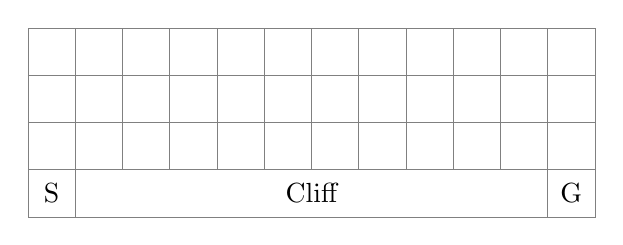
\begin{tikzpicture}[scale=0.60]
    \draw[gray,very thin] ( 0, 1) --
                          ( 0, 0) --
                          ( 1, 0) --
                          ( 1, 1);
    \draw[gray,very thin] ( 1, 0) -- (11, 0);
    \draw[gray,very thin] (11, 1) --
                          (11, 0) --
                          (12, 0) --
                          (12, 1);
    \draw[step=1cm,gray,very thin] (0, 1) grid (12, 4);
    \draw (0.5, 0.5) node {S};
    \draw (11.5, 0.5) node {G};
    \draw (6, 0.5) node {Cliff};
\end{tikzpicture}

\caption{Cliff walking environment.}
\label{fig:cliff_walking}
\end{figure}

Since the agent receives a reward of -1 for each time step, it is incentivized to reach the goal as fast as possible. Clearly, this implies that the optimal policy is the one that walks closest to the cliff, obtaining a cumulative reward of -13 for each episode.

\subsection{Frozen lake}
The frozen lake environment is a~${4\times4}$ grid in which the agent has to cross the frozen lake from a starting point~{(S)} to a goal~{(G)} while avoiding holes~{(H)}. The default configuration of the grid and the according optimal policy are shown in Figure~\ref{fig:frozen_lake}. Due to the slippery nature of the lake, the agent will move towards its intended direction with probability~${1/3}$, else it will move in either of the perpendicular directions with an equal probability of~${1/3}$. The reward is 1 if the agent reaches the goal, and 0 otherwise.
\begin{figure}
\centering
\begin{subfigure}{0.3\textwidth}
	\centering
	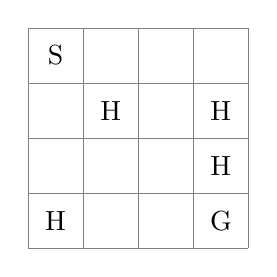
\begin{tikzpicture}[scale=0.7]
    \draw[step=1cm,gray,very thin] (0, 0) grid (4, 4);
    \draw (0.5, 3.5) node {S};
    \draw (0.5, 0.5) node {H};
    \draw (1.5, 2.5) node {H};
    \draw (3.5, 2.5) node {H};
    \draw (3.5, 1.5) node {H};
    \draw (3.5, 0.5) node {G};
\end{tikzpicture}

	\caption{Environment.}
\end{subfigure}
\begin{subfigure}{0.3\textwidth}
	\centering
	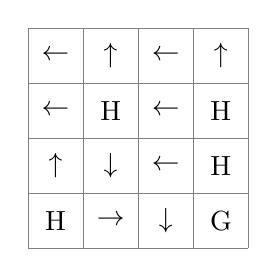
\begin{tikzpicture}[scale=0.7]
    \draw[step=1cm,gray,very thin] (0, 0) grid (4, 4);
    \draw (0.5, 3.5) node {$\leftarrow$};
    \draw (1.5, 3.5) node {$\uparrow$};
    \draw (2.5, 3.5) node {$\leftarrow$};
    \draw (3.5, 3.5) node {$\uparrow$};
    \draw (0.5, 2.5) node {$\leftarrow$};
    \draw (1.5, 2.5) node {H};
    \draw (2.5, 2.5) node {$\leftarrow$};
    \draw (3.5, 2.5) node {H};
    \draw (0.5, 1.5) node {$\uparrow$};
    \draw (1.5, 1.5) node {$\downarrow$};
    \draw (2.5, 1.5) node {$\leftarrow$};
    \draw (3.5, 1.5) node {H};
    \draw (0.5, 0.5) node {H};
    \draw (1.5, 0.5) node {$\rightarrow$};
    \draw (2.5, 0.5) node {$\downarrow$};
    \draw (3.5, 0.5) node {G};
\end{tikzpicture}

	\caption{Optimal policy.}
\end{subfigure}
\caption{Frozen lake environment.}
\label{fig:frozen_lake}
\end{figure}

Intuitively, the solution can be explained as follows: the best policy is to move in such a way that both the intended direction, as well as its perpendicular directions, do not result in falling into a hole. Thus, here the objective is to reach the goal as safely as possible, rather than as fast as possible.

\subsection{Mountain car}
In the mountain car environment~\cite{moore1990control} a car placed at the bottom of a valley has to reach a goal state on top of a hill. Due to the steepness of the valley, the car cannot simply accelerate forwards and reach the goal. Instead, it has to sway from one hill to the other until it has gained enough momentum to get to the top. Figure~\ref{fig:mountain_car} is a visual representation of the environment.
\begin{figure}
\centering
\begin{tikzpicture}
\begin{axis}[
    my full width, my samples,
    xmin=-1.2, xmax=0.6, ymin=0, ymax=1.2,
    x axis line style={draw=none},
    y axis line style={draw=none},
    xtick={\empty},
    ytick={\empty},
    scale only axis,
    axis equal image,
]
    % Hills
    \addplot+[semithick, draw=black, mark=none] {sin(deg(3 * x)) * 0.45 + 0.55};

    % Goal flag
    \draw (pi / 6, 1) -- (pi / 6, 1.2);
    \draw (pi / 6, 1.2) -- (pi / 6 + 0.05, 1.17);
    \draw (pi / 6 + 0.05, 1.17) -- (pi / 6, 1.14);

    % Car
    \pgfmathsetmacro{\carrotataion}{49}
    \pgfmathsetmacro{\carwidth}{0.17};
    \pgfmathsetmacro{\carheight}{0.1};
    \pgfmathsetmacro{\carposx}{-0.25};
    \pgfmathsetmacro{\carposy}{sin(deg(3 * \carposx)) * 0.45 + 0.55 + \carheight / 2 + 0.1};
    \draw[
        % rotate around={cos(deg(3 * \carposx)):(\carposx, \carposy)}
        rotate around={\carrotataion:(\carposx, \carposy)},
        draw=none,
        fill=black
    ]
        (\carposx - \carwidth / 2, \carposy - \carheight / 2) rectangle
        (\carposx + \carwidth / 2, \carposy + \carheight / 2);

    % Wheels
    \pgfmathsetmacro{\wheelradius}{0.03};
    \draw[
        rotate around={\carrotataion:(\carposx, \carposy)},
        draw=none,
        fill=gray
    ]
        (\carposx - \carwidth / 4, \carposy - \carheight / 2 - \wheelradius / 2)
        circle [radius=\wheelradius];
    \pgfmathsetmacro{\wheelradius}{0.03};
    \draw[
        rotate around={\carrotataion:(\carposx, \carposy)},
        draw=none,
        fill=gray
    ]
        (\carposx + \carwidth / 4, \carposy - \carheight / 2 - \wheelradius / 2)
        circle [radius=\wheelradius];
\end{axis}
\end{tikzpicture}

\caption{Mountain car environment.}
\label{fig:mountain_car}
\end{figure}

The state is a tuple containing the position of the car along the x-axis and the velocity of the car. There are two variants of the environment, the first one has~3 discrete actions (accelerate to the left, do not accelerate, accelerate to the right), whereas the second one takes as an action a value between~${\left[-1,1\right]}$ representing the directional force applied to the car. Additionally, in the continuous action space case, the car is penalized for taking actions of large magnitude. In both cases the maximum number of steps per episode has been set to~10000.

\section{Finite state space experiments}
We will now compare the theoretical results presented in the first two chapters, with empirical results obtained in these environments. We will also observe that even in such simple problems, both the choice of the method to be used, as well as its parameters, is not straightforward. In order to assess how well the reinforcement learning agents have trained, we will use the mean squared error between the optimal value, computed via dynamic programming, and the estimate value.

\subsection{Policy and value iteration}
We first present an example comparing policy and value iteration. We will consider the cliff walking problem. Since the the environment has a terminal state, we can also consider the case in which~${\discount=1}$.

Figure~\ref{fig:pi_convergence} presents the maximum change in the value function for each full sweep of the state space, for the first prediction step of policy iteration, with different discount values.
\begin{figure}
\centering
\begin{tikzpicture}
\begin{axis}[
    my cycle list, my axis, my scaling, my full width, my anchored legend,
    xlabel=Full sweeps of the state space,
    ylabel=${\left\lvert\left\lvert\estimatestatevalue-\estimatestatevalue'\right\rvert\right\rvert_{\infty}}$,
    xmin=1, xmax=1e5, ymin=1e-3, ymax=250,
    xmode=log, ymode=log,
]
    \addplot+ table[x=sweep, y=delta] {tikz/data/policy_iteration_delta/0_9.dat};
    \addlegendentry{$\discount=0.9$};

    \addplot+ table[x=sweep, y=delta] {tikz/data/policy_iteration_delta/0_95.dat};
    \addlegendentry{$\discount=0.95$};

    \addplot+ table[x=sweep, y=delta] {tikz/data/policy_iteration_delta/0_99.dat};
    \addlegendentry{$\discount=0.99$};

    \addplot+ table[x=sweep, y=delta] {tikz/data/policy_iteration_delta/1.dat};
    \addlegendentry{$\discount=1$};
\end{axis}
\end{tikzpicture}

\caption{Convergence rate for the first prediction step of policy iteration.}
\label{fig:pi_convergence}
\end{figure}
The learned policy is the same for each of the optimal value functions obtained with the various discount factors, yet the number of sweeps needed for the first prediction step varies widely. Table~\ref{tab:policy_iteration_convergence} illustrates this.
\begin{table}
\centering
\begin{tabular}{l c c}
\toprule
${\discount}$ & Avg. number of sweeps & Iterations \\
\midrule
0.9 & 63 & 13 \\
0.95 & 127 & 12 \\
0.99 & 282 & 9 \\
1 & 4298 & 9 \\
\bottomrule
\end{tabular}
\caption{Average number of sweeps in the prediction step of policy iteration and total number of iterations needed to converge to the optimal policy.}
\label{tab:policy_iteration_convergence}
\end{table}
Furthermore, as the discount factor gets smaller, each of the prediction steps is less precise, thus requiring more iterations in order to converge to the optimal policy.

Interestingly, policy iteration still converges to the optimal value function with~${\discount=1}$ when stopping the prediction step to a maximum upper bound of sweeps of the state space (e.g.,~100), clearly indicating that convergence in the prediction step is not always necessary to converge to the optimal policy.

In this problem, value iteration simply requires one iteration to converge to the optimal value. Of course, the initial value function and policy influence significantly the convergence rate of both methods.

\subsection{Scheduling strategies for~\texorpdfstring{${\varepsilon}$}{epsilon}}
We now move onto reinforcement learning methods. We will start by comparing different scheduling strategies for~${\varepsilon}$ with various methods. In figure~\ref{fig:epsilon_schedules} the schedules taken into consideration are shown.
\begin{figure}[ht]
\centering
\begin{tikzpicture}
\begin{axis}[
    my cycle list, my axis, my scaling, my full width, my anchored legend, my samples,
    xlabel={Episodes},
    ylabel={$\varepsilon$},
    xmin=0, xmax=30000, ymin=-0.01, ymax=1,
    domain=1:30000,
]
    \addplot+ {0.2};
    \addlegendentry{\small{Constant, $0.2$}};

    \addplot+ {0.8/(1+(1e-2*x))};
    \addlegendentry{\small{Linear, decay: $10^{-2}$}};

    \addplot+ {0.8/(1+(1e-3*x))};
    \addlegendentry{\small{Linear, decay: $10^{-3}$}};

    \addplot+ {0.8/(1+(1e-4*x))};
    \addlegendentry{\small{Linear, decay: $10^{-4}$}};
\end{axis}
\end{tikzpicture}

\caption{${\varepsilon}$~scheduling strategies taken into consideration.}
\label{fig:epsilon_schedules}
\end{figure}

Figure~\ref{fig:epsilon_frozen_lake} presents the mean squared error (MSE) between the optimal value and the estimate value at some episode for three reinforcement learning methods with the various scheduling strategies. The environment used here is the frozen lake problem. The results are averaged over~100 runs.
\begin{figure}
\centering
\begin{mseplot}{First-visit MC}{MSE}{10000}{6e-2}{}{0.24\linewidth}
\foreach \myepsilon in {{constant_0_2},{linear_1e-2},{linear_1e-3},{linear_1e-4}} {
	\addplot+ table[x=episode, y=mse] {tikz/data/epsilon/firstvisitmc_\myepsilon.dat};
}
\end{mseplot}
\begin{mseplot}{SARSA}{}{10000}{6e-2}{\empty}{0.24\linewidth}
\foreach \myepsilon in {{constant_0_2},{linear_1e-2},{linear_1e-3},{linear_1e-4}} {
	\addplot+ table[x=episode, y=mse] {tikz/data/epsilon/sarsa_\myepsilon.dat};
}
\end{mseplot}
\begin{mseplot}{Q-learning}{}{10000}{6e-2}{\empty}{0.24\linewidth}
\foreach \myepsilon in {{constant_0_2},{linear_1e-2},{linear_1e-3},{linear_1e-4}} {
	\addplot+ table[x=episode, y=mse] {tikz/data/epsilon/qlearning_\myepsilon.dat};
}
\end{mseplot}
\caption{MSE for various reinforcement learning methods with different scheduling strategies for~${\varepsilon}$.}
\label{fig:epsilon_frozen_lake}
\end{figure}

The first two cases, first-visit Monte Carlo and SARSA, require a GLIE sequence of policies in order to converge to the optimal value. Still, in this simple example even a constant~${\varepsilon}$ works adequately, even if the training the error does not decrease as quickly as in the case of the decaying schedules. Among GLIE policies certain decay values work better than others. Although this might also depend on the problem itself, it is mainly a byproduct of the chosen number of training episodes. A policy whose~${\varepsilon}$ decays too rapidly, such as the one with a decay of~${10^{-2}}$, will result in low exploration and, consequently, worse results. Vice versa, a policy which remains exploratory for too long does not allow to the agent to exploit what it has learned. Ultimately, we have Q-learning, which only needs that the state-action pairs continue to be visited to converge. As a result of this, the policy with the worst performance is once again the one with highest decay.

Figure~\ref{fig:epsilon_frozen_lake_variance} displays the MSE~$\pm$ the standard deviation across 10 runs, in the case of the policy with a decay rate of~${10^{-3}}$.
\begin{figure}
\centering
\begin{mseplot}{First-visit MC}{MSE}{10000}{6e-2}{}{0.24\linewidth}
    \pgfplotsset{cycle list shift=2}
    \addplot+ table [x=episode, y=mse] {tikz/data/epsilon/firstvisitmc_linear_1e-3.dat};
    \pgfplotsset{cycle list shift=1}
    \addplot+[solid, opacity=0.3, mark=none, name path=top] table [x=episode, y=top] {tikz/data/epsilon/firstvisitmc_linear_1e-3.dat};
    \pgfplotsset{cycle list shift=0}
    \addplot+[solid, opacity=0.3, mark=none, name path=bottom] table [x=episode, y=bottom] {tikz/data/epsilon/firstvisitmc_linear_1e-3.dat};
    \pgfplotsset{cycle list shift=-1}
    \addplot+[fill opacity=0.1] fill between[of=top and bottom];
\end{mseplot}
\begin{mseplot}{SARSA}{}{10000}{6e-2}{\empty}{0.24\linewidth}
    \pgfplotsset{cycle list shift=2}
    \addplot+ table [x=episode, y=mse] {tikz/data/epsilon/sarsa_linear_1e-3.dat};
    \pgfplotsset{cycle list shift=1}
    \addplot+[solid, opacity=0.3, name path=top] table [x=episode, y=top] {tikz/data/epsilon/sarsa_linear_1e-3.dat};
    \pgfplotsset{cycle list shift=0}
    \addplot+[solid, opacity=0.3, name path=bottom] table [x=episode, y=bottom] {tikz/data/epsilon/sarsa_linear_1e-3.dat};
    \pgfplotsset{cycle list shift=-1}
    \addplot+[fill opacity=0.1] fill between[of=top and bottom];
\end{mseplot}
\begin{mseplot}{Q-learning}{}{10000}{6e-2}{\empty}{0.24\linewidth}
    \pgfplotsset{cycle list shift=2}
    \addplot+ table [x=episode, y=mse] {tikz/data/epsilon/qlearning_linear_1e-3.dat};
    \pgfplotsset{cycle list shift=1}
    \addplot+[solid, opacity=0.3, name path=top] table [x=episode, y=top] {tikz/data/epsilon/qlearning_linear_1e-3.dat};
    \pgfplotsset{cycle list shift=0}
    \addplot+[solid, opacity=0.3, name path=bottom] table [x=episode, y=bottom] {tikz/data/epsilon/qlearning_linear_1e-3.dat};
    \pgfplotsset{cycle list shift=-1}
    \addplot+[fill opacity=0.1] fill between[of=top and bottom];
\end{mseplot}

\caption{MSE~$\pm$ the standard deviation across 10 runs for various reinforcement learning methods with~${\varepsilon}$ decaying at a rate of~${10^{-3}}$.}
\label{fig:epsilon_frozen_lake_variance}
\end{figure}
First-visit Monte Carlo, being a Monte Carlo method, is high variance due to the fact that the precision of its estimate depends on all the states, actions, and rewards in each episode. Here, since the episodes can be rather short, especially at the start of the training process, where the agent often falls in the hole, the difference in variance between the methods is not as remarkable.

Even in such a simple environment we can observe how scheduling strategies that should theoretically converge, may fail to do so in practice. Vice versa, with a constant value of~${\varepsilon}$ we obtained satisfactory results even though reinforcement learning theory says otherwise. Furthermore, such observations are obviously only possible where the optimal value can be computed, but in real-world scenarios, where the mean squared error cannot be estimated, the trained agents need to be evaluated separately.

\subsection{On- and off-policy learning}
We now present a further example in order to compare SARSA and Q-learning, on the cliff walking environment. Both methods are trained with a constant~${\varepsilon}$ of~{0.1}. The left part of Figure~\ref{fig:cliff_walking_on_off_policy_reward} shows the reward obtained for each of the~800 episodes of training.
\begin{figure}
\centering
\begin{tikzpicture}
\begin{axis}[
    my cycle list, my axis, my scaling,
    xlabel={Episodes},
    ylabel={Reward},
    xmin=0, xmax=800, ymin=-200, ymax=0,
    width=0.35\linewidth,
    scaled y ticks=false,
    legend style={at={(1,0)},anchor=south east,cells={anchor=west}},
]
    \addplot+ table [x=episode, y=reward] {tikz/data/cumulative_reward/sarsa_reward.dat};
    \addlegendentry{SARSA};

    \addplot+ table [x=episode, y=reward] {tikz/data/cumulative_reward/qlearning_reward.dat};
    \addlegendentry{Q-learning}
\end{axis}
\end{tikzpicture}

\begin{mseplot}{}{MSE}{800}{80}{}{0.35\linewidth}
    \addplot+ table [x=episode, y=mse] {tikz/data/cumulative_reward/sarsa_mse.dat};
    \addplot+ table [x=episode, y=mse] {tikz/data/cumulative_reward/qlearning_mse.dat};
\end{mseplot}
\caption{Reward (averaged over~100 runs and then smoothed with a moving average of~10 episodes) and MSE for each episode (averaged over~100 runs).}
\label{fig:cliff_walking_on_off_policy_reward}
\end{figure}

The rewards obtained during training also include rewards obtained after exploratory moves. These moves can sometimes also make the agent fall off the cliff when walking on its edge. Q-learning falls off more frequently since it directly learns the values of the optimal greedy policy, whereas SARSA takes a safer route by learning the values of the (approximately) optimal~${\varepsilon}$-greedy policy. This causes Q-learning to obtain less reward during training, even though it has learned to behave optimally, while SARSA obtains larger rewards as it walks farther away from the cliff.

Even though this example was specifically designed for this comparison, it makes apparent that in general the reward obtained during training is not a good proxy for how well the agent will do in the real environment. Furthermore, as exhibited in the right part of Figure~\ref{fig:cliff_walking_on_off_policy_reward}, the error of the two methods is almost identical, yet, due to the differences between the two detailed in the previous paragraph, Q-learning will always behave optimally, whereas SARSA will behave sub-optimally by being safer, obtaining a total reward of either -15 or -17.

\subsection{The choice of \texorpdfstring{${\robbinsmonro}$}{alpha}}
The TD update \eqref{eq:td_update} can be rearranged as follows:
\begin{align}
	\estimatestatevalue\left(\randomstate_{\timestep}\right)
		&\gets\estimatestatevalue\left(\randomstate_{\timestep}\right)+\robbinsmonro\left(\randomreward_{\timestep+1}+\discount\estimatestatevalue\left(\randomstate_{\timestep+1}\right)-\estimatestatevalue\left(\randomstate_{\timestep}\right)\right) \notag \\
		&=\estimatestatevalue\left(\randomstate_{\timestep}\right)-\robbinsmonro\estimatestatevalue\left(\randomstate_{\timestep}\right)+\robbinsmonro\left(\randomreward_{\timestep+1}+\discount\estimatestatevalue\left(\randomstate_{t+1}\right)\right) \notag \\
		&=\left(1-\robbinsmonro\right)\estimatestatevalue\left(\randomstate_{\timestep}\right)+\robbinsmonro\left(\randomreward_{\timestep+1}+\discount\estimatestatevalue\left(\randomstate_{\timestep+1}\right)\right).
\end{align}
When~${0<\robbinsmonro\leq1}$ we can interpret the step size parameter as the weight given between the old estimate of the value,~${\estimatestatevalue\left(\randomstate_{\timestep}\right)}$, and the new estimate of the value,~${\randomreward_{\timestep+1}+\discount\estimatestatevalue\left(\randomstate_{\timestep+1}\right)}$. Clearly, the value of~${\robbinsmonro}$, alongside its decay schedule, takes the role of the learning rate, as in supervised learning.

Figure~\ref{fig:alphas} presents the MSE~$\pm$ the standard deviation obtained training a SARSA agent on the frozen lake environment with different values of~${\robbinsmonro}$. The policy is linearly decaying with a decay of~${10^{-3}}$, starting from~0.8.
\begin{figure}
\centering
\begin{mseplot}{${\robbinsmonro}=0.01$}{MSE}{10000}{6e-2}{}{0.24\linewidth}
    \pgfplotsset{cycle list shift=2}
    \addplot+ table [x=episode, y=mse] {tikz/data/alpha/0_01_alpha.dat};
    \pgfplotsset{cycle list shift=1}
    \addplot+[solid, opacity=0.3, name path=top] table [x=episode, y=top] {tikz/data/alpha/0_01_alpha.dat};
    \pgfplotsset{cycle list shift=0}
    \addplot+[solid, opacity=0.3, name path=bottom] table [x=episode, y=bottom] {tikz/data/alpha/0_01_alpha.dat};
    \pgfplotsset{cycle list shift=-1}
    \addplot+[fill opacity=0.1] fill between[of=top and bottom];
\end{mseplot}
\begin{mseplot}{${\robbinsmonro}=0.15$}{}{10000}{6e-2}{\empty}{0.24\linewidth}
    \pgfplotsset{cycle list shift=2}
    \addplot+ table [x=episode, y=mse] {tikz/data/alpha/0_15_alpha.dat};
    \pgfplotsset{cycle list shift=1}
    \addplot+[solid, opacity=0.3, name path=top] table [x=episode, y=top] {tikz/data/alpha/0_15_alpha.dat};
    \pgfplotsset{cycle list shift=0}
    \addplot+[solid, opacity=0.3, name path=bottom] table [x=episode, y=bottom] {tikz/data/alpha/0_15_alpha.dat};
    \pgfplotsset{cycle list shift=-1}
    \addplot+[fill opacity=0.1] fill between[of=top and bottom];
\end{mseplot}
\begin{mseplot}{${\robbinsmonro}=0.30$}{}{10000}{6e-2}{\empty}{0.24\linewidth}
    \pgfplotsset{cycle list shift=2}
    \addplot+ table [x=episode, y=mse] {tikz/data/alpha/0_30_alpha.dat};
    \pgfplotsset{cycle list shift=1}
    \addplot+[solid, opacity=0.3, name path=top] table [x=episode, y=top] {tikz/data/alpha/0_30_alpha.dat};
    \pgfplotsset{cycle list shift=0}
    \addplot+[solid, opacity=0.3, name path=bottom] table [x=episode, y=bottom] {tikz/data/alpha/0_30_alpha.dat};
    \pgfplotsset{cycle list shift=-1}
    \addplot+[fill opacity=0.1] fill between[of=top and bottom];
\end{mseplot}

\caption{MSE (averaged over~100 runs)~$\pm$ the standard deviation (over~100 runs) with SARSA and different values of~${\alpha}$.}
\label{fig:alphas}
\end{figure}
Predictably, smaller values of~${\robbinsmonro}$ convergence steadily but slowly. Vice versa, larger values of~${\robbinsmonro}$ converge quickly, but with oscillations which might compromise the precision of the estimate. As usual, the parameter has to be manually tuned in order to achieve a good trade-off between the two.

\section{Continuous state space experiments}
We now proceed to the case of continuous state spaces, thus losing the possibility of using the mean squared error as a metric for how well the agent has trained. Instead, depending on the task, we will either use the steps or the reward per episode.

\subsection{Discretizing the state space}
We will start by taking the simple approach of discretizing the state space of the mountain car environment.

A total of~100 agents per discretization level have been trained, each for~500 episodes. Figure~\ref{fig:discretized_steps} shows the average steps per episode among all agents during the training process.
\begin{figure}
\centering
\begin{tikzpicture}
   \begin{axis}[
       my cycle list, my axis, my scaling, my full width, my anchored legend,
       xlabel=Episodes,
       ylabel=Steps,
       ytick={150, 500, 3000, 8000},
       ymode=log,
       xmax=500, ymin=100, ymax=8000,
       log ticks with fixed point,
   ]
       \addplot+ table [x=episode, y=steps] {tikz/data/discretized_state/5_bins.dat};
       \addlegendentry{5 bins};

       \addplot+ table [x=episode, y=steps] {tikz/data/discretized_state/10_bins.dat};
       \addlegendentry{10 bins};

       \addplot+ table [x=episode, y=steps] {tikz/data/discretized_state/20_bins.dat};
       \addlegendentry{20 bins};

       \addplot+ table [x=episode, y=steps] {tikz/data/discretized_state/40_bins.dat};
       \addlegendentry{40 bins};
   \end{axis}
\end{tikzpicture}

\caption{Steps per episode during training for various levels of discretization, smoothed with a moving average of~10 episodes.}
\label{fig:discretized_steps}
\end{figure}
At the end of each run of training, each agent was evaluated on~100 runs. Since the objective of the environment is for the car to reach the goal as fast as possible, we will use the steps to reach the goal on an episode as a metric to determine how well the agent has learned. Table~\ref{tab:discretized_eval} shows the results of this evaluations for each level of discretazation taken into consideration. In particular, we report the average number of steps and the standard deviation across all trained agents.
\begin{table}
\centering
\pgfplotstabletypeset[
	fixed,
	precision=0,
	columns={bins,avg_steps,std_dev_steps},
	display columns/0/.style={
		column name=Bins,
		column type={c},
		assign cell content/.code={
			\pgfkeyssetvalue{/pgfplots/table/@cell content}{##1$\times$##1}
		}
	},
	display columns/1/.style={
		column name=Average,
		column type={c},
	},
	display columns/2/.style={
		column name=Standard deviation,
		column type={c},
	},
	every head row/.style={
		before row={\toprule},
		after row={\midrule},
	},
	every last row/.style={
		after row={\bottomrule}
	}
]{tikz/data/eval_discrete.dat}
\caption{Steps to reach the goal across 100 runs of evaluation with different discretization levels.}
\label{tab:discretized_eval}
\end{table}

With both few and many bins we have middling results. In the first case the approximation is too coarse, whereas in the latter one the agents still needs more training episodes in order to fully explore the discretized state space. This environment is rather manageable, thus allowing good results even with few  bins and training episodes. A simple idea to adapt this method to more complex environments is that of discretizing the state space unevenly, in order to have finer discretization in parts of the state space which are more important.

Likely better results can be achieved by training for much longer and with many bins, but clearly this method does not scale well to problems with larger state spaces, as exploring them fully could prove to be too costly. Methods which update states not yet visited are needed instead.

\subsection{Tuning the features}
When using radial basis functions as features, we have to tune both the width of each feature, as well as the number of centers, or features. Larger values of~${\rbfwidth}$ result in smaller responses as the state gets farther from the center. To avoid having spots of the state space in which there is no response, we can increase the number of features which, of course, consequently makes the training harder. The centers of the features are sampled randomly. This might generate clusters of features in uninteresting parts of the state space, which can hinder learning. Notice that, as for the discritized case, if instead we had prior knowledge about the state space, we could place finer features in its most relevant portions, and coarser ones in less relevant ones.

We repeat the experiment of the previous section for different combinations of~$\rbfwidth$ and number of features. Figure~\ref{fig:features_steps} reports the steps per episode during training, while Table~\ref{tab:features_eval} reports results during evaluation.
\begin{figure}
\centering
% \begin{tikzpicture}
%     \begin{axis}[
%         my cycle list, my axis, my scaling,
%         title=${\rbfwidth=5}$,
%         xlabel=Episodes,
%         ylabel=Steps,
%         ytick={150, 500, 3000, 8000},
%         ymode=log,
%         xmax=500, ymin=100, ymax=8000,
%         log ticks with fixed point,
%         width=0.27\linewidth,
%     ]
%         \addplot+ table [x=episode, y=steps] {tikz/data/tuning_features/5_gamma_100_features.dat};
%         \addplot+ table [x=episode, y=steps] {tikz/data/tuning_features/5_gamma_500_features.dat};
%         \addplot+ table [x=episode, y=steps] {tikz/data/tuning_features/5_gamma_1000_features.dat};
%     \end{axis}
% \end{tikzpicture}
% \begin{tikzpicture}
%     \begin{axis}[
%         my cycle list, my axis, my scaling,
%         title=${\rbfwidth=10}$,
%         ytick={\empty},
%         ymode=log,
%         xmax=500, ymin=100, ymax=8000,
%         log ticks with fixed point,
%         xlabel=Episodes,
%         width=0.27\linewidth,
%     ]
%         \addplot+ table [x=episode, y=steps] {tikz/data/tuning_features/10_gamma_100_features.dat};
%         \addplot+ table [x=episode, y=steps] {tikz/data/tuning_features/10_gamma_500_features.dat};
%         \addplot+ table [x=episode, y=steps] {tikz/data/tuning_features/10_gamma_1000_features.dat};
%     \end{axis}
% \end{tikzpicture}
% \begin{tikzpicture}
%     \begin{axis}[
%         my cycle list, my axis, my scaling,
%         title=${\rbfwidth=25}$,
%         ytick={\empty},
%         ymode=log,
%         xmax=500, ymin=100, ymax=8000,
%         log ticks with fixed point,
%         xlabel=Episodes,
%         width=0.27\linewidth,
%         legend style={
%             font=\scriptsize,
%             at={(0.5,1)},
%             anchor=north,
%             cells={anchor=west}
%         },
%     ]
%         \addplot+ table [x=episode, y=steps] {tikz/data/tuning_features/25_gamma_100_features.dat};
%         \addlegendentry{100 features};
%         \addplot+ table [x=episode, y=steps] {tikz/data/tuning_features/25_gamma_500_features.dat};
%         \addlegendentry{500 features};
%         \addplot+ table [x=episode, y=steps] {tikz/data/tuning_features/25_gamma_1000_features.dat};
%         \addlegendentry{1000 features};
%     \end{axis}
% \end{tikzpicture}

\begin{tikzpicture}
    \begin{axis}[
        my cycle list, my axis, my scaling,
        title=100 features,
        xlabel=Episodes,
        ylabel=Steps,
        xtick={0,250,500},
        ytick={150, 500, 3000, 8000},
        ymode=log,
        xmax=500, ymin=100, ymax=8000,
        log ticks with fixed point,
        width=0.25\linewidth,
    ]
        \addplot+ table [x=episode, y=steps] {tikz/data/tuning_features/5_gamma_100_features.dat};
        \addplot+ table [x=episode, y=steps] {tikz/data/tuning_features/10_gamma_100_features.dat};
        \addplot+ table [x=episode, y=steps] {tikz/data/tuning_features/25_gamma_100_features.dat};
    \end{axis}
\end{tikzpicture}
\begin{tikzpicture}
    \begin{axis}[
        my cycle list, my axis, my scaling,
        title=500 features,
        xtick={0,250,500},
        ytick={\empty},
        ymode=log,
        xmax=500, ymin=100, ymax=8000,
        log ticks with fixed point,
        xlabel=Episodes,
        width=0.25\linewidth,
    ]
        \addplot+ table [x=episode, y=steps] {tikz/data/tuning_features/5_gamma_500_features.dat};
        \addplot+ table [x=episode, y=steps] {tikz/data/tuning_features/10_gamma_500_features.dat};
        \addplot+ table [x=episode, y=steps] {tikz/data/tuning_features/25_gamma_500_features.dat};
    \end{axis}
\end{tikzpicture}
\begin{tikzpicture}
    \begin{axis}[
        my cycle list, my axis, my scaling,
        title=1000 features,
        xtick={0,250,500},
        ytick={\empty},
        ymode=log,
        xmax=500, ymin=100, ymax=8000,
        log ticks with fixed point,
        xlabel=Episodes,
        width=0.25\linewidth,
        legend style={
            at={(0.5,1)},
            anchor=north,
            cells={anchor=west}
        },
    ]
        \addplot+ table [x=episode, y=steps] {tikz/data/tuning_features/5_gamma_1000_features.dat};
        \addlegendentry{${\rbfwidth=5}$};
        \addplot+ table [x=episode, y=steps] {tikz/data/tuning_features/10_gamma_1000_features.dat};
        \addlegendentry{${\rbfwidth=10}$};
        \addplot+ table [x=episode, y=steps] {tikz/data/tuning_features/25_gamma_1000_features.dat};
        \addlegendentry{${\rbfwidth=25}$};
    \end{axis}
\end{tikzpicture}

\caption{Steps per episode during training for different combinations of number and width of features, smoothed with a moving average of~10 episodes.}
\label{fig:features_steps}
\end{figure}
\begin{table}[ht]
\centering
\pgfplotstabletypeset[
	fixed,
	precision=0,
	columns={n_features,gamma,avg_steps,std_dev_steps},
	display columns/0/.style={
		column name=Features,
		column type={l},
		assign cell content/.code={
			\pgfmathparse{int(Mod(\pgfplotstablerow,3)}
			\ifnum\pgfmathresult=0
				\pgfkeyssetvalue{/pgfplots/table/@cell content}{\multirow{3}{*}{##1}}
			\else
				\pgfkeyssetvalue{/pgfplots/table/@cell content}{}
			\fi
		},
	},
	display columns/1/.style={
		column name=${\rbfwidth}$,
		column type={c},
	},
	display columns/2/.style={
		column name=Average,
		column type={c},
	},
	display columns/3/.style={
		column name=Standard deviation,
		column type={c},
	},
	every head row/.style={
		before row={\toprule},
		after row={\midrule},
	},
	every nth row={3}{
		before row={\midrule},
	},
	every last row/.style={
		after row={\bottomrule}
	}
]{tikz/data/eval_features.dat}
\caption{Steps to reach the goal across 100 runs of evaluation with different combinations of number and width of features.}
\label{tab:features_eval}
\end{table}
When the number of features is low, the features are too sparse to properly describe the state space. As the number of features increases, both the average steps episode and the standard deviation between the agents decrease. Perhaps surprisingly, the second-best average is obtained with many features of large width, which intuitively should result in many redundant features. Possibly, both fully covering the state space with large features, and partly covering the state space (i.e., only its most significant portions) with smaller features, produce similar outcomes. This hypothesis could also explain the slightly higher variance in the case of the parameters that yielded the lowest average, since the effectiveness of the trained agent would depend on where such features are placed.

\subsection{The \texorpdfstring{${\lambda}$}{lambda} parameter}
In the case of $n$-step methods and TD($\lambda$) we have a further tuning parameter indicating how farther back in the past each state has contributed to the reward obtained at the current time step. In the case of the mountain car environment, the car has to gather momentum. This process takes many time steps. Thus, previous states and actions have great importance when considering how to act in the present.

We once again repeat the same experiment with a SARSA(${\lambda}$) agent, using~500 features with a width of~10, as on average they yielded the best results in the previous section. Since the steps per episode during training are rather close in all cases, we only report the steps per episode during the evaluation process (Table~\ref{tab:lambda_eval}).
\begin{table}
\centering
\pgfplotstabletypeset[
	fixed,
	precision=0,
	columns={lambda,avg_steps,std_dev_steps},
	display columns/0/.style={
		column name=${\lambda}$,
		column type={l},
		precision=2,
	},
	display columns/1/.style={
		column name=Average,
		column type={c},
	},
	display columns/2/.style={
		column name=Standard deviation,
		column type={c},
	},
	every head row/.style={
		before row={\toprule},
		after row={\midrule},
	},
	every last row/.style={
		after row={\bottomrule}
	}
]{tikz/data/eval_lambda.dat}
\caption{Steps to reach the goal across~100 runs of evaluation for different values of~${\lambda}$.}
\label{tab:lambda_eval}
\end{table}

As we mentioned in Section~{\ref{sec:td_lambda}} in the case of~${n}$ for~{${n}$-step} methods, also in the case of~${\lambda}$ intermediate values produce better results. Here, we can also clearly notice how the value of~${\lambda}$ balances bias and variance. When~${\lambda=0}$ we bootstrap at each time step, and thus we have high bias. As~${\lambda}$ approaches~1 a larger amount of previous states and actions are taken into consideration when computing the current update, consequently increasing the variance.

\subsection{Comparison of approximate methods}
We will now compare some of the approximate methods introduced previously on the mountain car environment. We will once again use~500 features with a width of~10. Figure~\ref{fig:continuous_steps} shows the steps per episode during training, whereas Table~\ref{tab:continuous_eval} shows the steps per episode during evaluation.
\begin{figure}
\centering
\begin{tikzpicture}
    \begin{axis}[
        my cycle list, my axis, my scaling, my full width, my anchored legend,
        xlabel=Episodes,
        ylabel=Steps,
        ytick={150, 500, 3000, 8000},
        ymode=log,
        xmax=500, ymin=100, ymax=8000,
        log ticks with fixed point,
    ]
        \addplot+ table [x=episode, y=steps] {tikz/data/continuous_state/sarsa_continuous.dat};
        \addlegendentry{SARSA};

        \addplot+ table [x=episode, y=steps] {tikz/data/continuous_state/qlearning_continuous.dat};
        \addlegendentry{Q-learning};

        \addplot+ table [x=episode, y=steps] {tikz/data/continuous_state/actorcritic_continuous.dat};
        \addlegendentry{One-step actor-critic};
    \end{axis}
\end{tikzpicture}

\caption{Steps per episode during training for different methods, smoothed with a moving average of~10 episodes.}
\label{fig:continuous_steps}
\end{figure}
\begin{table}
\centering
\pgfplotstabletypeset[
	fixed,
	precision=0,
	columns={method,avg_steps,std_dev_steps},
    col sep=comma,
	display columns/0/.style={
		column name=Method,
		column type={l},
		string type,
	},
	display columns/1/.style={
		column name=Average,
		column type={c},
	},
	display columns/2/.style={
		column name=Standard deviation,
		column type={c},
	},
	every head row/.style={
		before row={\toprule},
		after row={\midrule},
	},
	every last row/.style={
		after row={\bottomrule}
	}
]{tikz/data/eval_continuous.dat}
\caption{Steps to reach the goal across~100 runs of evaluation with different methods.}
\label{tab:continuous_eval}
\end{table}

Although one-step actor-critic is initially lagging behind, during training the average steps per episode for all methods are very similar. Theoretically Q-learning has no guarantee of converging when approximating the value function, yet in practice, although worse than SARSA on average, it is able to reach satisfactory results. Additionally, while SARSA is slightly better than one-step actor-critic on average, the latter has a much lower variance, and achieves similar results for all trained agents.

\subsection{Continuous action space}
We now move onto the mountain car environment variant which has continuous actions. In this case the problem is much harder, as the agent has to not only reach the goal, but also to do so without making actions of large magnitude. As such, we report both the steps per episode and the reward per episode in Figures~\ref{fig:features_continuous_action_steps} and~\ref{fig:features_continuous_action_rewards}, and Table~\ref{tab:features_continuous_action}. 
\begin{figure}
\centering
\begin{tikzpicture}
    \begin{axis}[
        my cycle list, my axis, my scaling,
        title=100 features,
        xlabel=Episodes,
        ylabel=Steps,
        xtick={0,250,500},
        ytick={150, 500, 3000, 8000},
        ymode=log,
        xmax=500, ymin=100, ymax=8000,
        log ticks with fixed point,
        width=0.25\linewidth,
        legend style={
            at={(0,0)},
            anchor=south west,
            cells={anchor=west},
            % font=\scriptsize,
        },
    ]
        \addplot+ table [x=episode, y=steps] {tikz/data/features_continuous_action/5_gamma_100_features.dat};
        \addlegendentry{${\rbfwidth=5}$};
        \addplot+ table [x=episode, y=steps] {tikz/data/features_continuous_action/10_gamma_100_features.dat};
        \addlegendentry{${\rbfwidth=10}$};
        \addplot+ table [x=episode, y=steps] {tikz/data/features_continuous_action/25_gamma_100_features.dat};
        \addlegendentry{${\rbfwidth=25}$};
    \end{axis}
\end{tikzpicture}
\begin{tikzpicture}
    \begin{axis}[
        my cycle list, my axis, my scaling,
        title=500 features,
        xlabel=Episodes,
        xtick={0,250,500},
        ytick={\empty},
        ymode=log,
        xmax=500, ymin=100, ymax=8000,
        log ticks with fixed point,
        width=0.25\linewidth,
    ]
        % \addplot+ table [x=episode, y=steps] {tikz/data/features_continuous_action/5_gamma_500_features.dat};
        \pgfplotsset{cycle list shift=1}
        \addplot+ table [x=episode, y=steps] {tikz/data/features_continuous_action/10_gamma_500_features.dat};
        \addplot+ table [x=episode, y=steps] {tikz/data/features_continuous_action/25_gamma_500_features.dat};
    \end{axis}
\end{tikzpicture}
\begin{tikzpicture}
    \begin{axis}[
        my cycle list, my axis, my scaling,
        title=1000 features,
        xlabel=Episodes,
        xtick={0,250,500},
        ytick={\empty},
        ymode=log,
        xmax=500, ymin=100, ymax=8000,
        log ticks with fixed point,
        width=0.25\linewidth,
    ]
        % \addplot+ table [x=episode, y=steps] {tikz/data/features_continuous_action/5_gamma_1000_features.dat};
    	\pgfplotsset{cycle list shift=1}
        \addplot+ table [x=episode, y=steps] {tikz/data/features_continuous_action/10_gamma_1000_features.dat};
        \addplot+ table [x=episode, y=steps] {tikz/data/features_continuous_action/25_gamma_1000_features.dat};
    \end{axis}
\end{tikzpicture}

\caption{Steps per episode during training for different combinations of number and width of features, smoothed with a moving average of~10 episodes.}
\label{fig:features_continuous_action_steps}
\end{figure}
\begin{figure}[ht]
\centering
\begin{tikzpicture}
    \begin{axis}[
        my cycle list, my axis, my scaling,
        title=100 features,
        xlabel=Episodes,
        ylabel=Reward,
        xtick={0,250,500},
        xmax=500, ymin=-600, ymax=0,
        width=0.25\linewidth,
        legend style={
            at={(1,0)},
            anchor=south east,
            cells={anchor=west},
            % font=\scriptsize,
        },
    ]
        \addplot+ table [x=episode, y=reward] {tikz/data/features_continuous_action/5_gamma_100_features.dat};
        \addlegendentry{${\rbfwidth=5}$};
        \addplot+ table [x=episode, y=reward] {tikz/data/features_continuous_action/10_gamma_100_features.dat};
        \addlegendentry{${\rbfwidth=10}$};
        \addplot+ table [x=episode, y=reward] {tikz/data/features_continuous_action/25_gamma_100_features.dat};
        \addlegendentry{${\rbfwidth=25}$};
    \end{axis}
\end{tikzpicture}
\begin{tikzpicture}
    \begin{axis}[
        my cycle list, my axis, my scaling,
        title=500 features,
        xlabel=Episodes,
        xtick={0,250,500},
        ytick={\empty},
        xmax=500, ymin=-600, ymax=0,
        width=0.25\linewidth,
    ]
        %\addplot+ table [x=episode, y=reward] {tikz/data/features_continuous_action/5_gamma_500_features.dat};
        \pgfplotsset{cycle list shift=1}
        \addplot+ table [x=episode, y=reward] {tikz/data/features_continuous_action/10_gamma_500_features.dat};
        \addplot+ table [x=episode, y=reward] {tikz/data/features_continuous_action/25_gamma_500_features.dat};
    \end{axis}
\end{tikzpicture}
\begin{tikzpicture}
    \begin{axis}[
        my cycle list, my axis, my scaling,
        title=1000 features,
        xlabel=Episodes,
        xtick={0,250,500},
        ytick={\empty},
        xmax=500, ymin=-600, ymax=0,
        width=0.25\linewidth,
    ]
        % \addplot+ table [x=episode, y=reward] {tikz/data/features_continuous_action/5_gamma_1000_features.dat};
        \pgfplotsset{cycle list shift=1}
        \addplot+ table [x=episode, y=reward] {tikz/data/features_continuous_action/10_gamma_1000_features.dat};
        \addplot+ table [x=episode, y=reward] {tikz/data/features_continuous_action/25_gamma_1000_features.dat};
    \end{axis}
\end{tikzpicture}


\caption{Reward per episode during training for different combinations of number and width of features, smoothed with a moving average of~10 episodes.}
\label{fig:features_continuous_action_rewards}
\end{figure}
\begin{table}
\centering
\begin{tabular}{l l c c c c}
\toprule
Features & ${\sigma}$ & Average steps & SD steps & Average reward & SD reward \\
\midrule
\multirow{3}{*}{100} & 5 & 1870 & 414 & -98 & 40 \\
& 10 & 1576 & 187 & -66 & 19 \\
& 25 & 2525 & 241 & -155 & 25 \\
\midrule
\multirow{2}{*}{500} & 10 & 923 & 132 & -24 & 22 \\
& 25 & 1158 & 127 & -24 & 13 \\
\midrule
\multirow{2}{*}{1000} & 10 & 800 & 161 & -27 & 32 \\
& 25 & 1224 & 166 & -35 & 17 \\
\bottomrule
\end{tabular}
\caption{Steps to reach the goal and reward across~100 runs of evaluation for different combinations of number and width of features, smoothed with a moving average of 10 episodes.}
\label{tab:features_continuous_action}
\end{table}

A standard deviation of 1 for the Gaussian policy has been used. The cases in which the number of features is either 500 or 1000 and the width of the features 5 have been omitted, as even with different values of standard deviation of the Gaussian policy the agent was unable to learn properly. With a standard deviation of 1 the agent would often end up with a mean action which was of great magnitude, and a low probability of selecting a better choice and getting back on track. On the other hand, choosing higher values for the standard deviation rendered the learning slow and the results lackluster. This is likely an indication that parameterzing also the standard deviation, rather than only the mean, could be beneficial. However, the standard deviation is generally approximated as~${\sigma_{\policyparameter}\left(s\right)\doteq\exp\left(\featurevector\left(\state\right)^{\top}\policyparameter_{\sigma}\right)}$. This greatly limits the number of features that can be used, as the exponential can easily cause an overflow when all features have positive value (as is the case for RBFs).

The results obtained are rather similar to the ones in the case of a discrete action space (Table~\ref{tab:continuous_eval}). Of course, as the continuous action space variant is much harder, the number of average steps per episode is higher, but the ranking between each of the combinations of number and width of features is almost identical. It is also interesting to note that in all cases, the agents are able to learn to both reach the goal quickly and efficiently, without restricting themselves to learning just one or the other.
